%%%%%%%%%%%%%%%%%%%%%%%%%%%%%%%%%%%%%%%%%%%%%%%%%%%%%%%%%%%%%%%%%%%%%%%%%%%%%%%%
\chapter{Реализация генератора систем инструментирования}
%%%%%%%%%%%%%%%%%%%%%%%%%%%%%%%%%%%%%%%%%%%%%%%%%%%%%%%%%%%%%%%%%%%%%%%%%%%%%%%%

В данном разделе рассматривается реализация прототипа генератора систем автоматизации инструментирования программ.
Разработка и реализация осуществляется в соответствии с предложенным ранее подходом, рассмотренными ограничениями и поставленными требованиями.

%%%%%%%%%%%%%%%%%%%%%%%%%%%%%%%%%%%%%%%%%%%%%%%%%%%%%%%%%%%%%%%%%%%%%%%%%%%%%%%%
\section{Работа системы инструментирования}
%%%%%%%%%%%%%%%%%%%%%%%%%%%%%%%%%%%%%%%%%%%%%%%%%%%%%%%%%%%%%%%%%%%%%%%%%%%%%%%%

Для реализации прототипа генератора систем инструментирования был использован язык программирования C++ (в режиме соответствия стандарту C++17), а также возможности библиотек Boost~\cite{boost} версии <<1.72.0>>, argparse~\cite{argparse} и tinyxml2~\cite{tinyxml2} версий <<2.0>> и <<7.1.0>> соответственно.
Использование языка C++ совместно с перечисленными библиотеками позволяет создать, в некоторой мере, кросc-платформенный (Windows, Linux, Mac OS) инструмент для решения задачи инструментирования.
Далее будут рассмотрены основные детали реализации главных частей созданного прототипа.

%%%%%%%%%%%%%%%%%%%%%%%%%%%%%%%%%%%%%%%%
\subsection{Аннотация грамматики языка}
%%%%%%%%%%%%%%%%%%%%%%%%%%%%%%%%%%%%%%%%

В рамках обеспечения возможности составления пользовательской аннотации к предоставленной грамматике заданного целевого языка программирования в соответствии с этапом проектирования, описанным ранее, в реализованном прототипе генератора систем инструментирования был использован язык разметки XML.
В листинге~\ref{annotation-example} представлен пример части общей структуры файла аннотации для языка Python.

\begin{lstlisting}[frame=single, language=XML, label={annotation-example}, caption={Пример общей структуры файла аннотации.}]
<!-- default pipeline: txl "%SRC%" "%TRANSFORM%" -o "%DST%" %PARAMS% -->
<annotation
  pipeline='txl "%SRC%" "%ANNOTATION_DIR%/pyindent.txl" | txl stdin "%TRANSFORM%" -o "%DST%" %PARAMS%'
  >
  <grammar ...>...</grammar>
  <lib>...</lib>
  <points-of-interest>...</points-of-interest>
  <pointcuts>...</pointcuts>
</annotation>
\end{lstlisting}

Корневой XML-элемент (тег) $annotation$ имеет опциональный атрибут $pipeline$, предназначенный для построения высокоуровневых команд обработки исходных текстов.
В случае, когда атрибут $pipeline$ не представлен в тексте аннотации, его значение становится равным команде вида <<\lstinline{txl "%SRC%" "%TRANSFORM%" -o "%DST%" %PARAMS%}>>.

В реализованном прототипе генератора систем инструментирования для построения команд обработки исходных текстов были реализованы следующие текстовые метки-заполнители (placeholder):

\begin{itemize}[noitemsep]
  \item \textit{WORKING\_DIR}   -- путь к рабочей директории процесса генератора систем инструментирования.
  \item \textit{ANNOTATON\_DIR} -- путь к директории, которая содержит файл аннотации грамматики целевого языка программирования.
  \item \textit{SRC}            -- путь к исходному файлу с текстом на целевом языке программирования; инструментируемый текст программного обеспечения.
  \item \textit{DST}            -- путь к обработанному файлу с текстом на целевом языке программирования; инструментированный текст программного обеспечения.
  \item \textit{TRANSFORM}      -- путь к файлу с описанием на языке TXL синтезированных трансформаций предоставленного исходного текста программы.
  \item \textit{PARAMS}         -- дополнительные параметры для утилиты TXL; всегда включает параметр \lstinline{-i}, принимающий значение пути к директории, в которой содержится файл аннотации.
\end{itemize}

Кроме атрибута $pipeline$ корневой элемент содержит в себе следующие основные элементы:

\begin{itemize}[noitemsep]
  \item \textit{grammar}            -- высокоуровневое описание основных синтаксических конструкций целевого языка программирования в виде ориентированного графа (DAG).
  \item \textit{points-of-interest} -- информация, связанная с <<точками интереса>> (POI) -- выделенные пользователем пути к узлам дерева разбора, которые содержат наиболее полезные с точки зрения конечного пользователя данные, характеризующие как непосредственно точки инструментирования, так и некоторые промежуточные узлы.
  \item \textit{pointcuts}          -- информация, связанная с синтаксическими конструкциями целевого языка и точками инструментирования в них.
  \item \textit{lib}                -- дополнительные пользовательские вспомогательные TXL функции.
\end{itemize}

\nomenclature{DAG}{Directed Acyclic Graph -- ориентированный ациклический граф.}
\nomenclature{POI}{Point of Interest -- точка интереса.}

Далее будут более подробно рассмотрены перечисленные XML-элементы пользовательской аннотации для некоторой грамматики (грамматик).

%%%%%%%%%%%%%%%%%%%
\subsubsection{DAG ключевых типов узлов}
%%%%%%%%%%%%%%%%%%%

Рассмотрим реализованный способ высокоуровневого описания основных синтаксических конструкций целевого языка программирования.
В листинге~\ref{annotation-dag-example} представлен пример описания взаимосвязи ключевых синтаксических конструкций для языка Java (атрибут $language$).

\begin{lstlisting}[frame=single, language=XML, label={annotation-dag-example}, caption={Пример DAG для грамматики языка Java.}]
<grammar
  language="java"
  src="/grammar.txl"
  >
  <keyword-DAG>
    <package type="package_declaration">
      <imports type="repeat import_declaration"/>
      <class type="class_declaration">
        <method type="method_declaration">
          <if type="if_statement">
            <else type="else_clause"/>
          </if>
          <switch type="switch_statement">
            <case type="switch_alternative"/>
          </switch>
          <for type="for_statement"/>
          <while type="while_statement"/>
          <do_while type="do_statement"/>
          ...
        </method>
      </class>
    </package>
  </keyword-DAG>
</grammar>
\end{lstlisting}

В разработанном прототипе генератора систем инструментирования иерархические взаимосвязи между основными синтаксическими конструкциями и понятиями целевого языка программирования описываются в виде ориентированного ациклического графа (в данном случае -- дерева), вложенного в тело тега \textit{keyword-DAG} элемента $grammar$.
Имя каждого XML-элемента, вложенного в \textit{keyword-DAG} задает идентификатор синтаксической конструкции, а атрибут $type$ -- основной тип узла дерева разбора, который описывает эту синтаксическую конструкцию в соответствующей грамматике, относительный путь (относительно директории, содержащей аннотацию) к TXL-файлу которой задается с помощью атрибута $src$ основного элемента $grammar$.
Основной тип узла используется при построении различных TXL функций для фильтрации.
Описание остальных характеристик ключевых конструкций производится при объявлении существующих точек инструментирования.
Такое разделение было выполнено с учетом ручного составления файла аннотации, вследствие чего, содержимое тега \textit{keyword-DAG} играет роль однозначного отображения идентификаторов ключевых синтаксических конструкций в типы узлов грамматики целевого языка программирования.

%%%%%%%%%%%%%%%%%%%
\subsubsection{Описание POI}
%%%%%%%%%%%%%%%%%%%

В листинге~\ref{annotation-pois-example} приведен фрагмент аннотации для языка Java, в котором описываются несколько <<точек интереса>>, такие как (атрибут $id$) <<class\_name>> и <<if\_condition>>.

\begin{lstlisting}[frame=single, language=XML, label={annotation-pois-example}, caption={Пример описания <<точек интереса>>.}]
<points-of-interest>
...
  <point
    id="class_name"
    keyword="class"
    value-of="class_header:class_name"
    />

  <point
    id="if_condition"
    keyword="if"
    value-of="condition"
    />
...
\end{lstlisting}

В рассматриваемом примере точка интереса с идентификатором <<class\_name>> преобразуется в TXL функцию, исходный текст которой представлен в листинге~\ref{poi-src-example}.

\begin{lstlisting}[frame=single, language=TXL, label={poi-src-example}, caption={Пример синтезированной функции для точки интереса <<class\_name>>.}]
function __POI_get___POI_CLASS_NAME kw_Class [class_declaration]
  replace [stringlit]
    _ [stringlit]
  deconstruct kw_Class
    ClassHeader0 [class_header] _ [class_body]
  deconstruct ClassHeader0
    _ [repeat modifier] 'class ClassName1 [class_name] _ [opt extends_clause] _ [opt implements_clause]
  construct ClassName1_str [stringlit]
    _ [quote ClassName1]
  by
    ClassName1_str
end function
\end{lstlisting}

Синтез текста приведенной выше функции осуществляется с помощью предоставленной грамматики целевого языка программирования при поддержке со стороны составителя аннотации посредством указания последовательности и порядка узлов дерева разбора, которые необходимо извлечь и преобразовать в текстовый вид.
Более подробно этот процесс будет рассмотрен далее при описании процесса синтеза вспомогательных TXL-функций, а именно -- так называемых <<G-функций>>.

%%%%%%%%%%%%%%%%%%%
\subsubsection{Описание точек инструментирования}
%%%%%%%%%%%%%%%%%%%

Для описания остальной информации для каждой описываемой пользователем синтаксической конструкции используется набор XML-элементов, состоящий из тега $pointcuts$, содержащего несколько тегов $keyword$, равное числу описанных синтаксических конструкций.
В листинге~\ref{annotation-pointcuts-example} приведен пример описания в аннотации грамматики основной информации, связанной с понятием <<метода>> (атрибут $name$ тега $keyword$).

\begin{lstlisting}[frame=single, language=XML, label={annotation-pointcuts-example}, caption={Пример описания основной информации одной конструкции для языка Python.}]
<pointcuts>
  <keyword
    name="method"
    search-type="funcdef"
    sequential="false"
    >
    <templates>
      <template kind="replace">
        'def <!--id--> <!--parameters--> ': 'INDENT <!--newline-->
          <p name="before_body"/>
          <!--repeat statement_or_newline-->
          <p name="after_body"/>
        'DEDENT
      </template>

      <template kind="match">
        'def <!--id--> <!--parameters--> ': 'INDENT <!--newline-->
          <!--repeat statement_or_newline-->
        'DEDENT
      </template>
    </templates>
    <pointcuts>
      <pointcut name="before_body" clone="class::before_body"/>

      <pointcut name="after_body">
        <paste-algorithm>
          <fragment-to-variable
            name="Additions"
            type="repeat statement_or_newline"
            each-line-postfix="Newline"
            />
          <insert-call
            function="."
            params="Additions"
            />
        </paste-algorithm>
      </pointcut>
    </pointcuts>
  </keyword>
...
\end{lstlisting}

XML-элемент $keyword$ содержит в себе два взаимосвязанных тега, содержащих описание внешнего вида синтаксической конструкции и реализуемых в рамках этой конструкции точек вставки инструментирующего кода.
Необязательный атрибут $sequential$ используется для указания на необходимость интерпретации синтаксической конструкции как одного элемента или части последовательности.
В листинге~\ref{annotation-template-example} показан пример описания шаблона <<замены>> (атрибут $kind$).

\begin{lstlisting}[frame=single, language=XML, label={annotation-template-example}, caption={Пример описания шаблона.}]
<template kind="replace">
    'def <!--id--> <!--parameters--> ': 'INDENT <!--newline-->
        <p name="before_body"/>
        <!--repeat statement_or_newline-->
        <p name="after_body"/>
    'DEDENT
</template>
\end{lstlisting}

В разработанном прототипе были реализованы и активно используются два типа шаблонов:
\begin{itemize}[noitemsep]
  \item шаблон <<поиска>>
  \item шаблон <<замены>>
\end{itemize}

Шаблоны <<\underline{поиска}>> описывают некоторую структуру в виде набора терминалов и не-терминалов в терминах языка TXL (шаблон), который выступает образцом при проверке соответствия узла дерева разбора, инструментирование которого необходимо выполнить.

Терминальные символы оформляются с помощью обычного текста в соответствии с правилами экранирования языков TXL и XML (символ <<амперсанд>>, <<больше>>, <<меньше>>, одиночный символ <<кавычка>> перед спецсимволом и др.).

Нетерминальные символы (и соответствующие им названия типов узлов) оформляются в виде текста в XML-комментариях.
Названия переменных для соответствующих типов узлов будут сгенерированы автоматически на основании преобразования строки в <<Pascal-case>> вид и удаления всех пробельных символов.

Содержимое данного шаблона может быть сгенерировано автоматически из соответствующей грамматики языка программирования посредством указания в атрибуте \textit{auto-gen} значения <<grammar>>.

Шаблоны <<\underline{замены}>> описывают вид структуры, описанной в шаблоне <<поиска>> вместе с расстановкой точек инструментирования в виде XML-элементов $p$.
Единственным атрибутом этих элементов является название конкретной точки инструментирования, уникальное в пределах данного шаблона.

В листинге~\ref{annotation-algo-example} демонстрируются различные варианты описания упомянутых в шаблоне <<замены>> (листинг~\ref{annotation-template-example}) точек инструментирования.

\begin{lstlisting}[frame=single, language=XML, label={annotation-algo-example}, caption={Пример описания алгоритмов для точек инструментирования.}]
<pointcut name="before_body" clone="if::before_body"/>

<pointcut name="after_body">
    <paste-algorithm>
        <fragment-to-variable
          name="Additions"
          type="repeat statement_or_newline"
          each-line-postfix="Newline"
          />
        <insert-call
          function="."
          params="Additions"
          />
    </paste-algorithm>
</pointcut>
\end{lstlisting}

XML-элемент $pointcut$ описывает точку инструментирования, которая была упомянута в шаблоне <<замены>> для конкретной синтаксической конструкции языка программирования.

Атрибут $clone$ позволяет уменьшить дублирование одинаковых описаний алгоритмов работы для нескольких несвязанных точек инструментирования.
Значение этого атрибута указывает на точку-оригинал, алгоритм работы которой необходимо скопировать для текущей, посредством указания имени синтаксической конструкции/ключевого слова и названия точки инструментирования, привязанной к этой конструкции.
Имена синтаксической конструкции и точки инструментирования разделяются, согласно примеру, посредством двойного символа <<двоеточие>>.

Вложенный элемент \textit{paste-algorithm} описывает последовательность действий, которые необходимо выполнить, чтобы осуществить вставку текста фрагмента.
Алгоритм работы подразумевает вызов команд с требуемыми параметрами.
В случае, когда конечный пользователь при составлении правил инструментирования указывает необходимость вставки нескольких фрагментов одновременно (через запятую) в одной точке инструментирования, выполняется подготовка текстов всех фрагментов посредством подстановки передаваемых параметров в указанные параметры-заполнители, после чего тексты фрагментов объединяются и далее рассматриваются как один монолитный подготовленный фрагмент исходного кода.
Ниже перечислены команды, доступные пользователю (составителю аннотации) при описании алгоритма инструментирования, которые были реализованы в прототипе генератора систем инструментирования:

\begin{itemize}[noitemsep]
  \item \lstinline{insert-text (text)} --
  вставка текста, заданного в параметре $text$, без экранирования в точке инструментирования, а именно, в выражении секции $by$ синтезируемой функции инструментирования (I-функции).

  \item \lstinline{insert-call (function, params)} --
  вставка вызова (пользовательской, но не только) функции $function$ с параметрами $params$, разделенными символом пробела. Параметры будут вставлены как есть, что позволяет использовать ключевое слово $each$ языка TXL для поэлементной работы с последовательностями (массивами и списками).

  \item \lstinline{insert-fragment ([each-line-prefix], [each-line-postfix])} --
  вставка текста фрагмента в точке инструментирования. Для каждой строки текста фрагмента опционально может быть задан некоторый текст, добавляемый в начало \textit{each-line-prefix} и в конец \textit{each-line-postfix}.

  \item \lstinline{create-variable ([name], type, value)} --
  создание TXL переменной с типом $type$, значение которой задано текстом параметра $value$. Имя переменной будет сгенерировано автоматически из названия используемого типа, но также может быть указано вручную, используя параметр $name$.

  \item \lstinline{deconstruct-variable (type, variant)} --
  добавление в функцию инструментирования (I-функцию) конструкции TXL для декомпозиции переменной с типом $type$ в соответствии с грамматикой целевого языка программирования, используя вариант с номером $variant$, если TXL тип многозначен.

  \item \lstinline{fragment-to-variable (name, type, [each-line-prefix], [each-line-postfix])} --
  создание TXL переменной в теле I-функции с типом $type$ и именем $name$, которая содержит в себе текст добавляемого фрагмента программного кода. Как и функция \textit{insert-fragment}, команда позволяет для каждой строки добавляемого текста опционально задать <<префикс>> и <<постфикс>>.
\end{itemize}

В упомянутом случае (листинг~\ref{annotation-algo-example}) алгоритм работы состоит в том, чтобы создать новую переменную, содержащую экранированный исходный текст шаблона, после чего выполнить вызов встроенной функции среды TXL (<<точка>>), которая осуществляет склеивание последовательностей.

%%%%%%%%%%%%%%%%%%%
\subsubsection{Пользовательские функции}
%%%%%%%%%%%%%%%%%%%

Поскольку набор доступных стандартных функций среды исполнения утилиты TXL достаточно ограничен, для составления аннотаций в прототипе была реализована возможность описания пользователями (составителями) собственных вспомогательных функций на языке TXL, исходный код которых требуется добавить в синтезируемое описание трансформаций (<<систему инструментирования>>).
Такая возможность позволят пользователям объединять существующие стандартные возможности для реализации более гибких и специфичных для отдельных целевых языков программирования функций по обработке элементов этих языков.
В листинге~\ref{annotation-lib-example} приведен пример определения пользователем вспомогательной функции с именем <<addToImportsIfNotExists>> (атрибут $name$).

\begin{lstlisting}[frame=single, language=XML, label={annotation-lib-example}, caption={Пример описания вспомогательной функции.}]
<lib>
  <function
    name="addToImportsIfNotExists"
    apply="call"
    params="Addition:import_declaration"
    >
      <source>
        replace [repeat import_declaration]
          Imports [repeat import_declaration]
        deconstruct not * [import_declaration] Imports
          Addition
        by
          Imports [. Addition]
      </source>
  </function>
...
\end{lstlisting}

Из приведенного примера видно, что функции задаются при помощи тега $function$, а правила -- $rule$.

Атрибут $apply$ позволяет задать один из вариантов политики исполнения данной функции/правила:
\begin{itemize}[noitemsep]
  \item <<before-all>>  -- до всех цепочек инструментирования;
  \item <<after-all>>   -- после всех цепочек инструментирования;
  \item <<call>>        -- непосредственный вызов из алгоритма работы точки инструментирования или другой функции/правила;
\end{itemize}

Атрибут $params$ позволяет задать список формальных параметров, разделенный символом <<точка с запятой>>, и их типов для функции/правила.
Как видно из листинга~\ref{annotation-lib-example}, функция <<addToImportsIfNotExists>> имеет один параметр типа <<import\_declaration>> с именем <<Addition>>.

%%%%%%%%%%%%%%%%%%%%%%%%%%%%%%%%%%%%%%%%
\subsection{Фрагменты программного кода}
%%%%%%%%%%%%%%%%%%%%%%%%%%%%%%%%%%%%%%%%

Аналогично файлам аннотаций в реализованном прототипе генератора систем инструментирования был использован язык XML для оформления пользователями фрагментов программного кода, вставку которого необходимо выполнить в соответствии с поставленными перед пользователем задачами.
В листинге~\ref{fragment-example} приведен пример пользовательского параметризованного фрагмента программного кода на некотором целевом языке программирования (в данном случае -- Java).

\begin{lstlisting}[frame=single, language=XML, label={fragment-example}, caption={Пример пользовательского фрагмента.}]
<fragment language="java" name="logging_message">
  <dependencies>
    <required name="logging_imports"/>
    <required name="logging_fields"/>
  </dependencies>

  <code black-list="imports" params="message">
    iLogger.log(Level.FINE, <p id="message"/>);
  </code>
</fragment>
\end{lstlisting}

Из приведенного листинга видно, что фрагмент состоит из элемента $fragment$, именуется <<logging\_message>> (атрибут $name$) и предназначается для использования при инструментировании программного кода на языке Java (атрибут $language$).
При этом фрагмент вынуждает пользователя использовать данный фрагмент с некоторыми другими фрагментами с именами <<logging\_imports>> и <<logging\_fields>> соответственно при помощи элемента $dependencies$, содержащего перечисление фрагментов, от которых зависит корректность работы добавляемого этим фрагментом программного кода.
В прототипе была реализована работа только элемента $required$, означающая строгую зависимость от включения другого фрагмента с именем, указанным в атрибуте $name$.

Для использования передаваемых параметров, перечисление которых осуществляется через запятую в атрибуте $params$ элемента $code$, в тексте фрагмента необходимо указание пустого XML-тега $p$ с атрибутом $id$, в котором указывается идентификатор используемого параметра.
Любое вложенное содержимое тега $p$ при этом игнорируется.

%%%%%%%%%%%%%%%%%%%%%%%%%%%%%%%%%%%%%%%%
\subsection{Правила инструментирования}
%%%%%%%%%%%%%%%%%%%%%%%%%%%%%%%%%%%%%%%%

В соответствии с ранее описанными на этапе проектирования требованиями к языку описания правил инструментирования в прототипе генератора систем инструментирования был реализован предметно-ориентированный декларативный язык.
В качестве основы для создания языка для описания пользователем правил инструментирования рассматривались DSL таких проектов как Annotation File Utilities~\cite{jaif} и AspectJ~\cite{aspectj}.
На рис.~\ref{fig:layout-ruleset} приведен пример описания с указанием основных элементов пользовательских правил инструментирования с помощью разработанного языка с точки зрения конечного пользователя системы.
\nomenclature{DSL}{Domain-Specific Language -- предметно-ориентированный язык.}

\begin{figure}[!h]
  \centering
  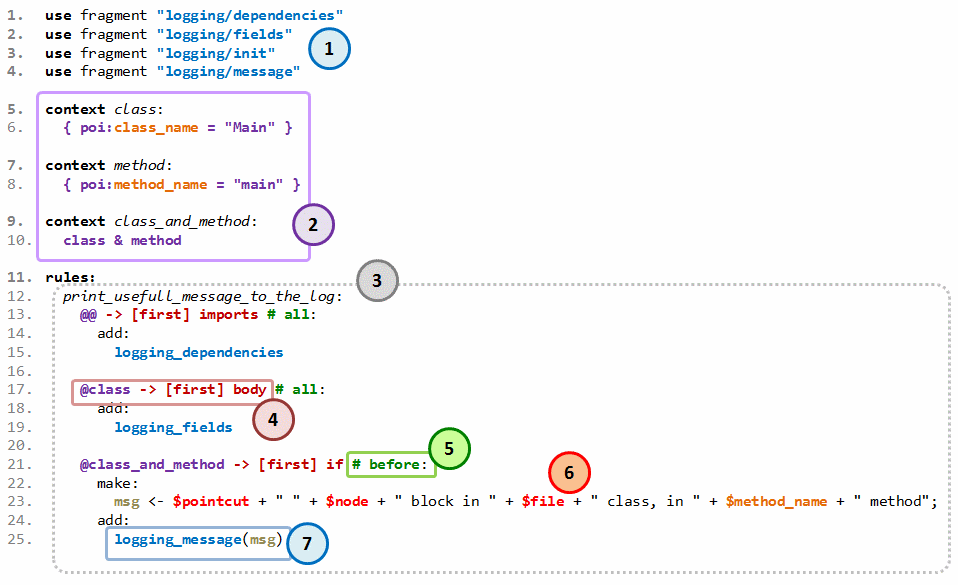
\includegraphics[width=4.2in]{layout_ruleset}
  \caption{Пример описания правил инструментирования.}
  \label{fig:layout-ruleset}
\end{figure}

Основными частями описания набора правил, в соответствии с реализованным в прототипе генератора систем инструментирования предметно-ориентированным языком, являются (номер пункта списка соответствует номеру на рис.~\ref{fig:layout-ruleset}):
\begin{enumerate}[noitemsep]
  \item перечисление используемых в данном наборе правил фрагментов исходных текстов и их относительное расположение в файловой системе;
  \item перечисление интересующих пользователя контекстов инструментирования;
  \item группировка этапов инструментирования в виде именованных правил;
  \item уточнение контекста инструментирования с применением ключевых слов языка программирования и текстовых шаблонов, если таковые требуются для целей уточнения контекста согласно решаемой пользователем задачи;
  \item указание одной конкретной точки инструментирования по ее идентификатору;
  \item создание пользовательских переменных из текстовых элементов и значений констант;
  \item список имен фрагментов, вставку которых необходимо выполнить одновременно в одном и том же месте, с указанием параметров, если таковые требуются согласно тексту используемого фрагмента.
\end{enumerate}

Из приведенного выше списка основных элементов видно, что разработанный язык полностью соответствует приведенным ранее требованиям.
Вместе с тем имеются возможности для дальнейшего усовершенствования.

Ключевыми особенностями являются два вида описания контекстов инструментирования ($2$) и возможность уточнения указанного контекста инструментирования ($4$, $5$).
Данные возможности позволяют пользователю достаточно точно ограничить область выполнения трансформаций, при этом скрывая от него детали реализации.
Важно отметить, что синтезируемые на выходе генератора описания трансформаций на языке TXL могут использоваться как стартовый шаблон для выполнения более сложных процедур инструментирования.

Для выполнения синтаксического разбора и анализа описаний на данном языке были использованы возможности утилиты TXL, такие как вывод дерева разбора в виде XML-дерева при передачи параметра \lstinline{-xml}.
Полный текст грамматики, описывающей синтаксис пользовательских правил инструментирования на языке TXL в данной работе рассмотрен не будет.
Дальнейший анализ был выполнен при помощи возможностей библиотеки tinyxml2.

%%%%%%%%%%%%%%%%%%%%%%%%%%%%%%%%%%%%%%%%
\subsection{Интерфейс командной строки}
%%%%%%%%%%%%%%%%%%%%%%%%%%%%%%%%%%%%%%%%

Реализованный прототип генератора систем инструментирования был реализован в виде однопоточного консольного приложения.
Для реализации интерфейса командной строки, а именно разбора параметров запуска исполнимого модуля, были использованы возможности библиотеки $argparse$~\cite{argparse}.
Данная библиотека позволяет в программном коде задавать используемые приложением параметры и одновременно с этим описывать это требование в виде текстовой пользовательской справки.

Ниже представлен список реализованных параметров запуска (в круглых скобках указано требование наличия):

\begin{itemize}[noitemsep]
  \item \lstinline{--src filenameI.lang}                -- (обязательно)
  путь к исходному файлу с текстом инструментируемого программного обеспечения, написанным на выбранном (целевом) языке программирования.

  \item \lstinline{--dst filenameO.lang}                -- (обязательно)
  путь к файлу, в котором будет сохранен инструментированный текст программы.

  \item \lstinline{--rule filename.dsl}                 -- (обязательно)
  путь к файлу, в котором описываются пользовательские правила инструметирования.

  \item \lstinline{--annotation filename.xml}           -- (обязательно)
  путь к файлу, содержащему аннотацию к грамматике, которая содержит описание конструкций языка программирования инструментируемого программного обеспечения.

  \item \lstinline{--fragments-dir /path/to/fragments/} -- (обязательно)
  путь к директории, который необходимо считать базовым при поиске используемых пользователем при описании правил инструментирования фрагментов текста на целевом языке программирования.

  \item \lstinline{--disable "rule_name_1;rule_name_2"} -- (опционально)
  разделенный символом <<точка с запятой>> список названий пользовательских правил инструментирования, которые необходимо игнорировать при синтезе описания трансформаций для утилиты TXL.

  \item \lstinline{--no-cache}         -- (опционально)
  игнорировать ранее сохраненные результаты синтеза пользовательского набора правил, если таковые имеются.

  \item \lstinline{--txl-params}       -- (опционально)
  дополнительные параметры для утилиты TXL, передаваемые на завершающем этапе -- при выполнении трансформаций.

  \item \lstinline{--scis-grm-ruleset} -- (обязательно)
  путь к грамматике, которая на языке TXL описывает структуру файлов с пользовательскими правилами инструментирования.
  \item \lstinline{--scis-grm-txl}     -- (обязательно)
  путь к грамматике, которая на языке TXL описывает сам язык TXL.
\end{itemize}

Параметры \lstinline{--scis-grm-ruleset} и \lstinline{--scis-grm-txl} используются для сокращения числа обращений к файловой системе в случае, если бы значения, задаваемые в этих параметрах, хранились бы в файлах настройки разработанного прототипа генератора систем инструментирования.

%%%%%%%%%%%%%%%%%%%%%%%%%%%%%%%%%%%%%%%%
\subsection{Обработка исключительных ситуаций}
%%%%%%%%%%%%%%%%%%%%%%%%%%%%%%%%%%%%%%%%

Помимо копирования файла с исходным текстом в качестве инструментированного, как было запланировано на этапе проектирования, для упрощения навигации пользователя в случаях наличия семантических ошибок в тексте описания пользовательских правил инструментирования в грамматику, при помощи которой выполняется разбор этого описания, были добавлены нетерминальные символы $srclinenumber$, которые позволяют сохранять номер строки в анализируемом тексте.
Номера строк выводятся в некоторых (в зависимости от контекста и доступности информации о номере строки) сообщениях об ошибках.
Неполная доступность информации о номере строки обосновывается тем, что данная функциональность была добавлена исключительно в демонстрационных целях.

%%%%%%%%%%%%%%%%%%%%%%%%%%%%%%%%%%%%%%%%%%%%%%%%%%%%%%%%%%%%%%%%%%%%%%%%%%%%%%%%
\section{Синтез цепочек TXL функций}
%%%%%%%%%%%%%%%%%%%%%%%%%%%%%%%%%%%%%%%%%%%%%%%%%%%%%%%%%%%%%%%%%%%%%%%%%%%%%%%%

Для реализации описанного ранее подхода к решению задачи инструментирования в разработанном прототипе генератора систем инструментирования была реализована функциональность по автоматической генерации описания трансформаций в виде набора взаимосвязанных TXL-функций.
В текущей версии прототипа этот процесс жестко фиксирован, но может быть подвергнут расширению и модернизации в будущих версиях.
Генерация TXL функций выполняется в соответствии со следующим алгоритмом:

\begin{enumerate}[noitemsep]
  \item загрузка, разбор и проверка зависимостей указанных фрагментов программного кода в соответствии с предоставленным описанием правил инструментирования;
  \item расчет максимальных расстояний для каждого узла направленного ациклического графа ключевых конструкций целевого языка программирования в соответствии с предоставленной аннотацией грамматики;
  \item построение оберток над стандартными \textit{текстовыми} операциями сравнения (W-функции);
  \item построение функций для реализации функциональности точек интереса (G-функции);
  \item построение функций проверки принадлежности узлов CST контекстам инструментирования (H-функции);
  \item построение цепочек функций в соответствии с правилами инструментирования с учетом значения аргумента командной строки \lstinline{--disable};
  \item построение вспомогательных TXL функций;
  \item построение дополнительных пользовательских функций и правил, взятых из секции $lib$ аннотации грамматики;
  \item построение главной TXL функции <<main>> и применение политик использования дополнительных пользовательских функций;
  \item обновление состояний функций, которые являются элементами цепочек;
  \item генерация TXL кода -- описания требуемых трансформаций, совместно с предоставленной грамматикой и средой исполнения TXL, являющегося системой инструментирования в соответствии с пользовательскими правилами.
\end{enumerate}

Важно отметить, что этап расчета максимального удаления для каждого узла DAG ключевых конструкций производится с помощью BFS-подобного алгоритма с применением очереди и ограниченного максимальным количеством итераций (2500 в разработанном прототипе).

Цепочки вызовов функций запускаются посредством прямого вызова первых функций в главной функции с именем <<main>>, где  основным параметром всегда является корневой элемент конкретного дерева разбора с типом $program$.
Результаты работы первой цепочки функций передаются последующим далее одна за другой.
В листинге~\ref{main-example} приведен пример исходного текста функции <<main>>.
Символ <<...>> содержат имена функций, которые были сокращены для повышения удобочитаемости.

\begin{lstlisting}[frame=single, language=TXL, label={main-example}, caption={Пример исходного текста главной функции.}]
function main
  replace [program]
    Program [program]
  by
    Program
    [..._refiner_imports_first0]
    [..._refiner_class_level0__helper]
    [..._collector_class_and_method_m_633_uid5]
    [..._collector_class_and_method_m_633_uid8]
    [simplify]
end function
\end{lstlisting}

Связывание нескольких TXL функций в единую последовательность было реализовано посредством наследования предметно-ориентированных типов функций от класса <<CallChainElement>>, описание которого приведено в листинге~\ref{chain-element-sample}.

\begin{lstlisting}[frame=single, language=C, label={chain-element-sample}, caption={Исходный код определения элемента цепочки вызовов.}]
struct CallChainElement {
  /// calleR
  TXLFunction const* callFrom = nullptr;
  /// calleE
  TXLFunction const* callTo = nullptr;
}; // CallChainElement
\end{lstlisting}

Ниже представлена общая структура типичной цепочки вызовов программно-синтезируемых предметно-ориентированных функций:
\begin{enumerate}[noitemsep]
  \item C-функции -- функции сбора информации (одна или несколько; может отсутствовать).
  \item F-функция -- функция фильтрации (одна; может отсутствовать).
  \item R-функций -- функций уточнения контекста (одна или несколько).
  \item I-функция -- функция инструментирования.
\end{enumerate}

Кроме этого используются следующие вспомогательные автоматически-синтезируемые TXL функции:
\begin{itemize}
  \item G-функции -- функции получения узлов, содержащих полезные значения (так называемых \textit{точек интереса}), из промежуточных узлов дерева разбора, имеющих TXL тип, который описывает какую-либо важную синтаксическую конструкцию целевого языка программирования.
  \item H-функции -- функции проверки принадлежности определенному контексту по передаваемым параметрам.
  \item W-функции -- функции-обертки стандартных операторов сравнения и поиска, выполняемых над текстовыми данными.
\end{itemize}

Синтез цепочек функций в разработанном прототипе производится для каждого пользовательского правила (пункт 3 на рис.~\ref{fig:layout-ruleset}) и для каждого отдельного выражения, содержащего уточнение контекста и ключевое слово $add$ вместе со списком фрагментов, в отдельно взятом правиле в порядке описания.

Далее будут рассмотрены перечисленные выше типы функций более подробно.

%%%%%%%%%%%%%%%%%%%%%%%%%%%%%%%%%%%%%%%%
\subsection{Функции сбора информации}
%%%%%%%%%%%%%%%%%%%%%%%%%%%%%%%%%%%%%%%%

Синтез цепочек функций для выполнения инструментирования начинается со сбора и упорядочения в порядке увеличения показателя максимального расстояния до корневого узла от узла, указанного как часть описания синтаксической конструкции целевого языка программирования.
Этот процесс осуществляется, основываясь на используемых указанным контекстом инструментирования синтаксических конструкциях.
Общее количество синтезированных C-функций в цепочке соответствует количеству требуемых источников данных для определения принадлежности узла выбранному контексту.

В соответствии с рассмотренной ранее методикой определения контекста, в прототипе генератора систем инструментирования был реализован процесс генерации так называемых C-функций и F-функций.
Функции фильтрации далее будут рассмотрены более подробно.

C-функции (англ. $collect$, $crawl$) -- это TXL функции, специализированные по типу обрабатываемых узлов дерева разбора, предназначенные для накопления информации из узлов древа разбора, которая впоследствии используется для определения, соответствует-ли рассматриваемый/обрабатываемый конечный узел дерева разбора выбранному контексту инструментирования.

Принцип работы таких функций заключается в вызове следующей функции из цепочки с передачей ей всех значений аргументов, которые были получены текущей, вместе с текущим рассматриваемым узлом, тип которого содержит необходимые сведения для дальнейших операций, таких как определение соответствия контексту и формирование значений для пользовательских переменных, используемых при заполнении указанного пользователем фрагмента исходного кода.

C-функции опираются на специфику работы функций-правил~(rule) языка TXL: правилу $R_{(T,P)}$ будут даны на рассмотрение все узлы текущего поддерева $G_{sub}$, соответствующие заявленному типу $T$ и сопоставимые шаблону $P$.

В листинге~\ref{cfunc-example} приведен пример исходного TXL кода простой C-функции с именем \lstinline{CollectorFuncB}, которая получает в виде аргумента некоторый узел с типом \lstinline{class_declaration}, выполняет копирование обрабатываемого узла с типом \lstinline{method_declaration} и передает эти данные (два узла, переданный в аргументах и обрабатываемый) следующей функции по цепочке вызовов с именем \lstinline{CollectorFuncC}.

\begin{lstlisting}[frame=single, language=TXL, label={cfunc-example}, caption={Пример синтезированной C-функции.}]
rule CollectorFuncB kw_Class [class_declaration]
  skipping [method_declaration]
  replace $ [method_declaration]
    __NODE__ [method_declaration]
  by
    __NODE__ [CollectorFuncC kw_Class __NODE__]
end rule
\end{lstlisting}

Стоит отметить, что существуют различные подходы к решению задачи передачи информации по цепочке функций:
\begin {itemize}[noitemsep]
  \item аргументы функций
    \begin{itemize}[noitemsep]
      \item добавление новых аргументов в конец (слева направо);
      \item добавление новых аргументов в начало (справа налево);
    \end{itemize}
  \item глобальные переменные;
  \item использование средств ввода-вывода среды TXL для временного хранения результатов во внешнем, родительском для утилиты TXL, процессе.
\end{itemize}

Как видно из приведенного примера (листинг~\ref{cfunc-example}), для реализации синтеза C-функций в разработанном прототипе был выбран первый способ передачи данных о необходимых узлах дерева разбора -- посредством аргументов функций, где новые узлы добавляются в конец списка.

Ограничения описанного выше способа организации сбора информации об узлах дерева разбора, примененного в разработанном прототипе генератора систем инструментирования:
\begin{itemize}[noitemsep]
  \item Синтаксическое дерево исходного текста программы не содержит циклов по типам узлов -- при спуске от корня к листьям каждый \textit{сохраняемый} тип узла встречается не более одного раза.
  \item Используемые типы узлов имеют строгую последовательность вложенности относительно друг друга (для узлов с одинаковым уровнем вложенности необходимо использовать R-функции, которые будут рассмотрены более детально далее).
  \item Невозможно выполнить сбор данных, не связанных напрямую с точкой, в которой необходимо выполнить инструментирование, или с одним из упомянутых узлов, состоящих в иерархии (цепочке) сохраняемых.
  \item Принятие решения о принадлежности узла контексту инструментирования осуществляется только в условиях полной доступности каждого сохраняемого типа узла дерева разбора.
\end{itemize}

%%%%%%%%%%%%%%%%%%%%%%%%%%%%%%%%%%%%%%%%
\subsection{Функции фильтрации по контексту}
%%%%%%%%%%%%%%%%%%%%%%%%%%%%%%%%%%%%%%%%

F-функции (англ. $filter$) -- это TXL функции, специализированные по типу обрабатываемых узлов дерева разбора, предназначенные для фильтрации узлов CST дерева разбора относительно описываемых конечным пользователем контекстов инструментирования.
Последняя C-функция в цепочке выполняет вызов F-функции, для корректной работы которой (определение принадлежности контексту) был выполнен сбор данных.
F-функция создается только при использовании определяемого пользователем контекста инструментирования.
Фильтрация осуществляется с помощью выражения $where$ и вызова соответствующей указанному контексту H-функции с передачей ей данных, собранных с помощью C-функций и полученных с помощью аргументов.
Более подробно синтез и работа H-функций рассмотрена далее.

В листинге~\ref{ffunc-example} приведен пример функции фильтрации по принадлежности контексту с именем <<context\_c\_and\_m>>.

\begin{lstlisting}[language=TXL, label={ffunc-example}, caption={Пример синтезированной F-функции.}]
function ..._filter_class_and_method674_uid9 kw_Class [class_declaration] kw_Method [class_declaration]
  replace $ [method_declaration]
    __NODE__ [method_declaration]
  construct __VOID__ [any]
    % void
  where
    __VOID__ [belongs_to_context_c_and_m kw_Class kw_Method]
  by
    __NODE__ [..._refiner_method_first0_uid10__starter kw_Class kw_Method]
end function
\end{lstlisting}

В случае указания в качестве контекста инструментирования специального идентификатора глобального контекста <<@>>, сбор информации и синтез C- и F-функций не производится.
В таком случае началом порождаемой цепочки является первая R-функция в соответствии с выражением, описываемым пользователем в пункте 4 из рис.~\ref{fig:layout-ruleset}.

%%%%%%%%%%%%%%%%%%%%%%%%%%%%%%%%%%%%%%%%
\subsection{Функции уточнения контекста}
%%%%%%%%%%%%%%%%%%%%%%%%%%%%%%%%%%%%%%%%

После проверки контекста функцией-фильтром происходит вызов первой функции из последовательности R-функций.

R-функции (англ. $refine$) -- это TXL функции, специализированные по типу обрабатываемых узлов дерева разбора, предназначенные для уточнения контекста до какой-либо требуемой синтаксической конструкции целевого языка программирования.
В листинге~\ref{rfunc-example} приведен пример исходного текста синтезированной R-функции.

\begin{lstlisting}[frame=single, language=TXL, label={rfunc-example}, caption={Пример синтезированной R-функции.}]
function refinerFunction kw_Class [class_declaration] kw_Method [class_declaration]
  replace * [repeat declaration_or_statement]
    __NODE__ [if_statement] __TAIL__ [repeat declaration_or_statement]
  construct __SINGLE_BOX_ARRAY__ [repeat declaration_or_statement]
    __NODE__ % +empty
  construct __PROCESSED__ [repeat declaration_or_statement]
    __SINGLE_BOX_ARRAY__ [instrumentationFunction kw_Class kw_Method]
  by
    __PROCESSED__ [. __TAIL__]
end function
\end{lstlisting}

Структура синтезированной R-функции варьируется в зависимости от нескольких факторов.
Одним из них является способ интерпретации единичного узла заданного типа в дереве разбора: как \underline{один элемент} или как \underline{член последовательности}.
Даже если используемый тип обрабатываемого узла содержит TXL модификаторы <<list>> или <<repeat>>, этот элемент будет интерпретирован в соответствии с указаниями составителя аннотации (по-умолчанию -- как один элемент).
Вариант <<член последовательности>> полезен в случаях, когда программисту запрещается правилами целевого языка программирования использование блоков кода в середине последовательности команд из внешнего блока кода, как, например, в языке Python.

Кроме того, вид и структуру порождаемой R-функции определяет используемый модификатор, указываемый пользователем при составлении правил инструментирования.
В разработанном прототипе были реализованы следующие модификаторы для уточняющих функций:

\begin{itemize}[noitemsep]
  \item \underline{first} -- поиск и обработка только самого \textit{первого} встреченного узла из текущего поддерева разбора в соответствии с типом, заданным в аннотации грамматики при описании синтаксической конструкции целевого языка программирования;
  \item \underline{all}   -- поиск и обработка \textit{всех узлов} в соответствии с типом, заданным в аннотации грамматики при описании синтаксической конструкции целевого языка программирования;
  \item \underline{level} -- поиск и обработка узлов, находящихся на \textit{одном уровне} (первом) вложенности таких узлов друг в друга.
\end{itemize}

Рассмотрим влияние различных модификаторов на поведение R-функций на примере небольшой программы на языке Python, исходный текст которой приведен в листинге~\ref{py-before-example-src}.
Для этого опишем набор правил инструментирования, каждое правило которого позволит легко выявить используемый модификатор.
Для этого воспользуемся реализованным в прототипе генератора идентификатором $std:rule$, который позволяет сохранить в пользовательской константе название текущего правила.
Полный текст составленного описания приведен в листинге~\ref{py-rules-example}.

\begin{lstlisting}[frame=single, label={py-rules-example}, caption={Применение различных модификаторов уточняющих функций в описании правил (форматирование изменено для компактности).}]
use fragment "frag"

rules:
  mod_1_FIRST:
    @@ -> [first] if # before:
      make:  msg <- $std:rule;
      add:   frag(msg)

  mod_2_ALL:
    @@ -> [all] if # before:
      make:  msg <- $std:rule;
      add:   frag(msg)

  mod_3_LEVEL:
    @@ -> [level] if # before:
      make:  msg <- $std:rule;
      add:   frag(msg)

  multiplie_LEVELs:
    @@ -> [level] if -> [level] if # before:
      make:  msg <- $std:rule;
      add:   frag(msg)
\end{lstlisting}

\begin{lstlisting}[frame=single, language=Python, label={py-before-example-src}, caption={Пример исходной программы на языке Python.}]
def test():
  if lvl == 11:
    if lvl == 22:
      if lvl == 33:
        print "Hello World!"
      
      if lvl == 33:
        print "Hello World!"
    
    if lvl == 22:
      if lvl == 33:
        print "Hello World!"
      
      if lvl == 33:
        print "Hello World!"
...
\end{lstlisting}

В листинге~\ref{py-after-example-src} приведен текст обработанной программы, текст которой был инструментирован в соответствии с описанными правилами.

\begin{lstlisting}[frame=single, language=Python, label={py-after-example-src}, caption={Результат применения различных модификаторов к исходной программе.}]
def test() :
    print "mod_1_FIRST"
    print "mod_2_ALL"
    print "mod_3_LEVEL"
    if lvl == 11 :
        print "mod_2_ALL"
        print "multiplie_LEVELs"
        if lvl == 22 :
            print "mod_2_ALL"
            if lvl == 33 :
                print "Hello World!"

            print "mod_2_ALL"
            if lvl == 33 :
                print "Hello World!"

        print "mod_2_ALL"
        print "multiplie_LEVELs"
        if lvl == 22 :
            print "mod_2_ALL"
            if lvl == 33 :
                print "Hello World!"

            print "mod_2_ALL"
            if lvl == 33 :
                print "Hello World!"
...
\end{lstlisting}

Результат применения различных модификаторов наглядно демонстрирует успешное выполнение операции инструментирования для
\textit{первой} синтаксической конструкции (вывод строки <<mod\_1\_FIRST>>),
\textit{всех} синтаксических конструкций (вывод строки <<mod\_2\_ALL>>),
синтаксических конструкций \textit{первого уровня} (вывод строки <<mod\_3\_LEVEL>>) и
совместного использования \textit{нескольких уровней} синтаксической конструкции (вывод строки <<multiplie\_LEVELs>>).

Перед кодированием каждого из перечисленных выше модификаторов R-функций необходимо было решить соответствующую смыслу данного модификатора задачу.

Для реализации модификатора \textbf{first} достаточно было воспользоваться стандартной особенностью языка TXL, которая именуется <<searching-function>>~\cite{txl-book} или <<поисковая функция>>/<<функция поиска>>.
Данная особенность заключается в создании TXL-функции в форме обыкновенной функции (используя ключевое слово $function$) и использовании символа-модификатора <<*>> одновременно с ключевым словом $replace$.
Алгоритм работы такой функции состоит в поиске первого подходящего под заданный шаблон узла дерева разбора.

Для реализации модификатора \textbf{all} стандартного решения найдено не было, вследствие чего была составлена упрощенная модель задачи следующего вида:

Пусть имеется слад $S$ и производственная линия $P$.
Склад вмещает некоторый каким-то образом структурированный набор различных <<контейнеров>> (коробки, грузовые контейнеры, шкатулки и т.д.).
При этом в одном <<контейнере>> может быть ноль или несколько других <<контейнеров>> (иерархия вложенности).
В качестве исполнителей присутствуют курьер и работник, выдающий и принимающий <<контейнеры>>.
Работник склада и курьер могут одновременно работать только с одним <<контейнером>>.
Работа курьера начинается и заканчивается на складе $S$.
Задача курьера состоит в передаче всех \underline{красных коробок} из склада $S$ для обработки на производственную линию $P$ и возврате результата обратно на склад $S$, при чем каждая красная коробка должна быть <<обработана>> только один раз.
Для этого ему требуется принять решение: доставить текущий <<контейнер>> на производственную линию или нет.
Отправленный на производственную линию $P$ <<контейнер>> $B_{in}$ при возврате помещается в некоторый дополнительный <<контейнер>> $\hat{B} \ni B_{in}$.

Для решения поставленной задачи с учетом особенностей языка TXL (ранний выход из функции/правила; последовательность обхода) был составлен следующий алгоритм принятия решения:

\begin{itemize}[noitemsep]
  \item Имеется глобальный счетчик <<число ``контейнеров'' для пропуска>>, $C \leftarrow 0$.
  \item Осуществляется один проход по всем <<контейнерам>>.

  \item повторять пока не будут пройдены работником все <<контейнеры>>:
    \begin{enumerate}[noitemsep]
      \item Предоставленный курьеру <<контейнер>> $B_{in}$ -- это коробка? Если нет -- возврат $B_{in}$.
      \item Коробка $B_{in}$ имеет красный цвет? Если нет -- возврат $B_{in}$.
      \item Скопировать текущее значение $C$ как $C_0$.
      \item Если $C > 0$, то обновить $C \leftarrow C_0 - 1$.
      \item Если $C_0 > 0$ -- возврат $B_{in}$.
      \item Отправить <<контейнер>> $I$ для обработки на производственную линию $P$.
      \item Получить обратно обработанный <<контейнер>> $B_{out} = \hat{B}$.
      \item Обновить $C \leftarrow 1$.
      \item Вернуть <<контейнер>> $B_{out}$ работнику склада $S$.
    \end{enumerate}
\end{itemize}

При возврате красная коробка $B_{in}$ помещается в некоторый дополнительный <<контейнер>>, вследствие чего при возврате на склад $S$ коробка $B_{in}$ будет впоследствии предоставлена курьеру повторно.
Для предотвращения повторной обработки одной и той же красной коробки $B_{in}$ используется счетчик $C$, который позволяет пропустить первую встреченную курьером подходящую коробку.

Представленное решение имеет один критический недостаток -- работа никогда не будет завершена в случае, если на производственной линии $P$ в <<контейнер>> добавляется одна или несколько новых красных коробок.

Данный алгоритм был реализован в виде TXL правила (функция, объявленная с помощью ключевого слова $rule$), выполняющего один проход (использование символа <<\$>> одновременно с ключевым словом $replace$~\cite{txl-book}) по поддереву.

Для реализации модификатора \textbf{level} был реализован аналогичный описанному выше (модификатор <<all>>) подход с небольшим отличием.
На рис.~\ref{fig:modifier_level_a} и \ref{fig:modifier_level_b} показаны обобщенные примеры, демонстрирующие оказываемое модификатором <<level>> влияние на поведение уточняющей функции.
\begin{figure}[!h]
  \centering
  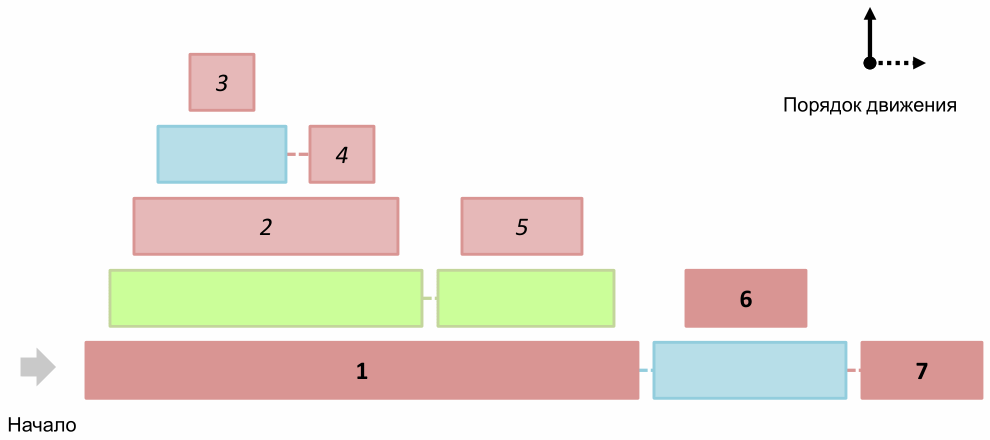
\includegraphics[width=3.2in]{modifier_level_a}
  \caption{Пример применения модификатора <<level>>.}
  \label{fig:modifier_level_a}
\end{figure}
\begin{figure}[!h]
  \centering
  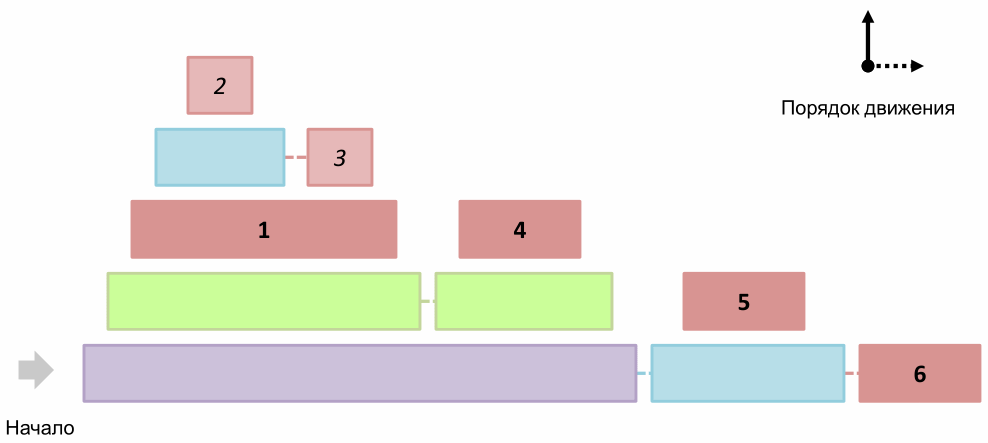
\includegraphics[width=3.2in]{modifier_level_b}
  \caption{Пример применения модификатора <<level>>.}
  \label{fig:modifier_level_b}
\end{figure}
Красным цветом выделены <<целевые>> объекты, тип которых требуется обработать.
Жирным выделены номера только тех объектов, которые соответствуют выражению <<\textit{первый уровень вложенности красных объектов друг в друга}>>.
В соответствии с этим, алгоритм принятия решения <<курьера>> был несколько модифицирован.

Этап 8 в данной задаче состоит в обновлении счетчика $C$ путем подсчета всех красных коробок в возвращаемом <<контейнере>>, $C~\leftarrow~counter(B_{out})$.

В соответствии с этим в прототипе был реализован синтез вспомогательных функций для подсчета узлов дерева разбора с указанным типом (<<красных коробок>>) вместе с функциями по уменьшению значения в счетчике (вследствие ограничений языка TXL).
В листинге~\ref{rfunc-counter-example-src} показан пример исходного текста функции-счетчика.
В данном случае глобальной переменной-счетчиком является \lstinline{__SKIP__1}.

\begin{lstlisting}[frame=single, language=TXL, label={rfunc-counter-example-src}, caption={Пример синтезированной функции-счетчика.}]
rule ..._refiner_if_level1_uid7_red_box_counter
	replace $ [if_statement]
		__NODE__ [if_statement]
	import __SKIP__1 [number]
	export __SKIP__1
		__SKIP__1 [+ 1]
	by
		__NODE__
end rule
\end{lstlisting}

В дополнение к перечисленному выше для каждой R-функции, содержащей модификатор, генерируется вспомогательная <<стартовая>> функция, принимающая рассматриваемый уровнем выше узел и проводящая инициализацию переменной-счетчика $C$ для реализаций модификаторов, подобных <<all>> и <<level>>.

Помимо модификаторов, R-функции способны осуществлять фильтрацию узлов на основании данных, извлекаемых из соответствующих точек интереса, которые были указаны при описании синтаксической конструкций целевого языка в аннотации грамматики.
Фильтрация осуществляется посредством проверки соответствия данных, представленных в точке интереса и текстового шаблона, задаваемого пользователем при составлении правил инструментирования.

В листинге~\ref{rfunc-pattern-example} приведен пример фрагмента из пользовательского описания правил инструментирования, в котором демонстрируется использование модификаторов совместно с фильтрацией по шаблону.
В листинге~\ref{rfunc-pattern-example-src} приведен соответствующий исходный текст синтезированной основной R-функции.

\begin{lstlisting}[frame=single, label={rfunc-pattern-example}, caption={Пример использования текстового шаблона.}]
...
  @class_and_method_m -> [first] method("m*ai*n") # before_body:
    add:
      logging_init
...
\end{lstlisting}

\begin{lstlisting}[frame=single, language=TXL, label={rfunc-pattern-example-src}, caption={Пример синтезированной R-функции со встроенной проверкой на соответствие шаблону.}]
function ..._refiner_method_first0_uid10 kw_Class [class_declaration] kw_Method [method_declaration]
  replace * [method_declaration]
    __INPUT__ [method_declaration]
  deconstruct __INPUT__
    __NODE__ [method_declaration]
  construct value_holder__uid11 [stringlit]
    _ [__POI_get___POI_METHOD_NAME __NODE__]
  construct S1_uid12 [stringlit]
    value_holder__uid11
  construct S1_uid12_LEN [number]
    _ [# S1_uid12]
  construct S1_uid12_POS [number]
    _ [index S1_uid12 "m"] 
  where %% starts with
    S1_uid12_POS [= 1]
  construct S2_uid12 [stringlit]
    S1_uid12 [: S1_uid12_POS S1_uid12_LEN]
  construct S2_uid12_LEN [number]
    _ [# S2_uid12]
  construct S2_uid12_POS [number]
    _ [index S2_uid12 "ai"] 
  where %% middle
    S2_uid12_POS [> 0]
  construct S3_uid12 [stringlit]
    S2_uid12 [: S2_uid12_POS S2_uid12_LEN]
  construct S3_uid12_LEN [number]
    _ [# S3_uid12]
  construct S3_uid12_POS [number]
    _ [index S3_uid12 "n"] [- 1] [+ 1]
  where %% ends with
    S3_uid12_POS [= S3_uid12_LEN]
  construct __OUTPUT__ [method_declaration]
    __INPUT__ [..._instrummenter_before_body_uid13 kw_Class kw_Method]
  by
    __OUTPUT__
end function
\end{lstlisting}

Комментарии, отделенные символами <<\%\%>>, рядом с директивой $where$ указывают на проверку условий, соответствующих описываемому текстовому шаблону.
Вначале выполняется извлечение данных из обрабатываемого узла дерева разбора в соответствии с указанной в аннотации точкой интереса при помощи синтезированной ранее G-функции (подробнее о них далее) с именем <<\_\_POI\_get\_\_\_POI\_METHOD\_NAME>>.
Извлеченные данные сохраняются в переменной <<value\_holder\_\_uid11>> для выполнения дальнейшего анализа.
Анализ извлеченной строки, в данном случае, заключается в следующем:

\begin{enumerate}[noitemsep]
  \item проверка и удаление фрагмента <<m>> в начале строки;
  \item проверка существования и удаление фрагмента <<ai>> где-то в оставшейся части строки;
  \item проверка существования фрагмента <<n>> в конце оставшейся строки.
\end{enumerate}

В завершении, обычно (в зависимости от интерпретации вида конструкции целевого языка программирования), создается переменная, содержащая результат работы следующей функции в цепочке и заменяющая текущий обрабатываемый узел дерева разбора.

%%%%%%%%%%%%%%%%%%%%%%%%%%%%%%%%%%%%%%%%
\subsection{Функции инструментирования}
%%%%%%%%%%%%%%%%%%%%%%%%%%%%%%%%%%%%%%%%

После выполнения процедуры уточнения контекста с помощью последовательности R-функций, последнее поддерево разбора (узел) передается на завершающий этап в конец цепочки исполнения для выполнения инструментирования.

I-функции (англ. $instrument$) -- это TXL функции, специализированные по типу обрабатываемых узлов дерева разбора, предназначенные непосредственно для выполнения инструментирования в соответствии с указанными в аннотации шаблонами (поиска и замены) и алгоритмом работы.
В листинге~\ref{ifunc-example} приведен пример исходного текста I-функции.
Синтез I-функции опирается на указанный пользователем в пункте пункте 5 рис.~\ref{fig:layout-ruleset} идентификатор точки инструментирования.

\begin{lstlisting}[frame=single, language=TXL, label={ifunc-example}, caption={Пример синтезированной I-функции.}]
function ..._instrummenter_before_uid12 kw_Class [class_declaration] kw_Method [method_declaration]
  replace $ [statement]
    __NODE__ [if_statement]
  deconstruct __NODE__
    'if '( Condition [condition] ') Statement [statement]
    OptElseClause [opt else_clause]
  import TXLinput [stringlit]
  construct STD_POINTCUT [id]     'before
  construct STD_NODE [id]         _ [typeof __NODE__]
  construct STD_FILE [stringlit]  _ [+ TXLinput]
  construct STD_RULE [id]         'print_usefull_message_to_the_log
  construct POI_METHOD_NAME [stringlit]
    _ [__POI_get___POI_METHOD_NAME kw_Method]
  construct POI_CLASS_NAME [stringlit]
    _ [__POI_get___POI_CLASS_NAME kw_Class]
  construct msg [stringlit]
    _ [+ STD_POINTCUT] [+ " <"] [+ STD_NODE] [+ "> block in ["] [+ POI_CLASS_NAME] [+ "] class, in {"] [+ POI_METHOD_NAME] [+ "} method"]
  by
    '{
      'iLogger.log(Level.FINE, msg ');     % <- from fragment
      'if '( Condition ') '{ Statement '}
      OptElseClause
    '}
end function
\end{lstlisting}

Рассматриваемая I-функция, как и (почти) все расположенные ранее в цепочке, получает собранную информацию о контексте инструментирования из передаваемых аргументов, в данном случае -- узлы с типами <<class\_declaration>> и <<method\_declaration>>.
Далее производится проверка обрабатываемого узла в соответствии с указанными в аннотации грамматики основным и вспомогательным (<<поисковым>>) типами, заданными для указанной синтаксической конструкции.
После чего выполняется проверка соответствия шаблону <<поиска>>, описанному в аннотации.
Если вышеперечисленные действия выполняются успешно, производится создание стандартных констант, содержащих такие данные как:

\begin{itemize}[noitemsep]
  \item $std:pointcut$  -- имя точки инструментирования;
  \item $std:node$      -- тип обрабатываемого узла дерева разбора;
  \item $std:file$      -- полное имя файла (при помощи импорта встроенной глобальной переменной языка TXL -- $TXLinput$);
  \item $std:rule$      -- пользовательское название правила инструментирования, в рамках которого применяется данная I-функция;
\end{itemize}

Кроме перечисленных выше создаются константы, содержащие значения, извлеченные из собранных данных, которые были переданы в передаваемых посредством аргументов функции узлах CST.
Константы создаются только по требованию в соответствии с использованием идентификаторов POI при создании определяемых пользователем переменных/констант.
Этот этап подразумевает сбор всех используемых идентификаторов <<точек интереса>> в выражениях, описывающих значения, которые должны принимать пользовательские константы.
Таким образом, имея полный список уникальных имен POI, создаются соответствующие переменные, выраженные в виде TXL кода, использующего директиву $construct$.
После чего аналогично создаются непосредственно определяемые пользователем константы.
Финальным этапом осуществляется замена входного узла в соответствии с шаблоном <<замены>>, описанном в аннотации грамматики, и алгоритмом инструментирования, выполняемым в месте, которое занимает указанная пользователем точка инструментирования.

Важно отметить, что в реализованном прототипе генератора систем инструментирования <<точки интереса>>, указанные пользователем при создании собственных переменных/констант, \textbf{не оказывают влияния} на генерацию C-функций и добавление новых узлов в аргументы промежуточных функций при движении по цепочке.
Руководствуясь этим фактом, рекомендуется использовать при необходимости ключевое слово $exists$ при описании контекстов инструментирования, где требуются данные, содержащиеся в соответствующих POI.
Данное недостаток также накладывает ограничение в виде невозможности определения каких-либо параметров узлов, упомянутых при выполнении уточнения контекста, типы которых совпадают или не могут быть выведены напрямую из определения контекста.

%%%%%%%%%%%%%%%%%%%%%%%%%%%%%%%%%%%%%%%%
\subsection{Вспомогательные TXL функции}
%%%%%%%%%%%%%%%%%%%%%%%%%%%%%%%%%%%%%%%%

Далее будут рассмотрены некоторые из вспомогательных TXL-функций, создаваемых генератором систем инструментирования автоматически при синтезе описания трансформаций.

%%%%%%%%%%%%%%%%%%%
\subsubsection{H-функции}
%%%%%%%%%%%%%%%%%%%

H-функции (англ. $help$) -- это TXL функции, специализированные по типам обрабатываемых узлов дерева разбора, предназначенные для проверки принадлежности определенному контексту узла дерева разбора по передаваемым параметрам.
Данный тип функций генерируется исходя из составленной конечным пользователем формулы при объявлении контекста в описании правил инструментирования, которая проходит процесс преобразования в форму КНФ.
Как уже было упомянуто ранее, язык TXL позволяет описывать ограничения в виде различных форм директивы $where$~\cite{txl-book}.
Одной из форм является ДНФ-подобная форма, однако она ограничена невозможностью использовать группировку выражений с помощью скобок и проверкой свойств только одной переменной, что в комбинации с поведением нескольких последовательно расположенных директив $where$ позволяет описывать логические выражения, представленные в КНФ форме.
Ограничение на одну переменную обходится при помощи создания переменной-<<затычки>>, имеющей тип <<any>> и содержащей мусорное значение (или отсутствие значения), и применения оберток над стандартными операторами проверки значений (W-функции; рассмотрено далее).
\nomenclature[0]{КНФ}{конъюнктивная нормальная форма.}
\nomenclature[0]{ДНФ}{дизъюнктивная нормальная форма.}

В соответствии с описанным выше принципом производится синтез функций этого типа в разработанном прототипе генератора систем инструментирования.
В листинге~\ref{hfunc-example} приведен пример H-функций с именами \lstinline{__belongs_to_context___namespace_m} и \lstinline{__not__belongs_to_context___namespace_m}.

\begin{lstlisting}[frame=single, language=TXL, label={hfunc-example}, caption={Пример синтезированной H-функций.}]
function __belongs_to_context___namespace_m kw_Method [procedure_impl_decl]
  match [any]
    _ [any]
  construct __VOID__ [any]
    % void
  construct POI_METHOD_NAMESPACE_str [stringlit]
    _ [__POI_get___POI_METHOD_NAMESPACE kw_Method]
  where
    __VOID__ [__std__equal POI_METHOD_NAMESPACE_str "Main."]
end function


function __not__belongs_to_context___namespace_m kw_Method [procedure_impl_decl]
  match [any]
    _ [any]
  construct __VOID__ [any]
    % void
  where not
    __VOID__ [__belongs_to_context___namespace_m kw_Method]
end function
\end{lstlisting}

Функция \lstinline{__belongs_to_context___namespace_m}, как видно из ее названия, реализует проверку принадлежности некоторого узла дерева разбора, который содержит данные с типом \textit{procedure\_impl\_decl}.
Другая же функция с именем \lstinline{__not__belongs_to_context___namespace_m} выполняет проверку \underline{не}соответствия выбранному контексту.

Извлечение данных перед проверкой значений производится при помощи вспомогательных G-функций, которые будут более подробно рассмотрены далее.

Для осуществления удобного построения цепочек из H-функций каждая из них принимает на вход в качестве основного проверяемого узел с любым типом (<<any>>), данные которого впоследствии полностью игнорируются.

Процесс синтеза H-функций различается в зависимости от типа описываемого контекста инструментирования:
простой контекст и
составной контекст.

Синтез H-функции для \underline{простого} контекста осуществляется посредством сбора информации об используемых точках интереса, указанных пользователем при составлении ограничений, описывающих этот тип контекста.
После сбора и порождения переменных, временно хранящих извлеченные данные (в соответствии с аннотацией и грамматикой), выполняется проверка указанных ограничений с использованием последовательности директив $where$.
Исходя из этого, отдельные ограничения объединяются логическим оператором $AND$, что означает принадлежность узла дерева разбора описываемому контексту только в случае удовлетворения всех наложенных ограничений/условий.
В случае использования пользователем текстового сопоставления шаблону, развертка инструкций по проверке осуществляется в рамках одной H-функции.

Синтез H-функции для \underline{составного} контекста осуществляется после обработки всех простых контекстов с учетом зависимостей текущего.
В случае если один или несколько зависимостей текущего еще не были созданы в виде H-функций, обработка текущего откладывается (используя очередь) с переходом к следующему составному контексту для обработки.
Обработка контекстов завершается при достижении пустой очереди или исчерпании лимита попыток создания, заданного в соответствии с формулой $T_{max}=N^2/2-1$ (где $T_{max}$ -- максимальное время работы (число итераций), $N$ -- число контекстов, от которых зависит текущий контекст), исходя из оценки худшего случая, когда зависимости представлены в порядке, обратном их созданию.
Вместе с тем, исчерпание этого лимита позволяет вынести решение об использовании пользователем несуществующего контекста или неверно заданной формулировкой.
В данном случае синтез H-функции производится в соответствии с КНФ формой, образуемой из описывающего контекст пользовательского выражения.

%%%%%%%%%%%%%%%%%%%
\subsubsection{G-функции}
%%%%%%%%%%%%%%%%%%%

G-функции (англ. $get$) -- это TXL функции, специализированные по типу обрабатываемых узлов дерева разбора, предназначенные для получения узлов, содержащих полезные значения, из промежуточных узлов дерева разбора, имеющих TXL тип, который описывает какую-либо важную синтаксическую конструкцию целевого языка программирования.

В листинге~\ref{gfunc-example} приведен пример G-функции, которая производит извлечение полного названия метода из узла с типом \textit{procedure\_impl\_decl}, представляющим описание метода в конкретном дереве разбора.

\begin{lstlisting}[frame=single, language=TXL, label={gfunc-example}, caption={Пример синтезированной G-функции.}]
function __POI_get___POI_METHOD_NAME_FULL kw_Method [procedure_impl_decl]
  replace [stringlit]
    _ [stringlit]
  deconstruct kw_Method
    ProcedureIntfDecl0 [procedure_intf_decl] _ [nested_decl_block] _ [procedure_body_semi]
  deconstruct ProcedureIntfDecl0
    ProcedureSignature1 [procedure_signature] _ [repeat semi_directive] _ [opt ';]
  deconstruct ProcedureSignature1
    _ [opt 'class] _ [procedure_keyword] ProcedureId2 [opt procedure_id] _ [opt formal_parameters] _ [opt colon_type]
  construct ProcedureId2_str [stringlit]
    _ [quote ProcedureId2]
  by
    ProcedureId2_str
end function
\end{lstlisting}

Структура G-функции определяется в соответствии с описанием пути $P$ и типом узла $T$ дерева разбора, указанными при описании <<точки интереса>> в аннотации грамматики.
В данном случае в аннотации для POI с именем <<method\_name\_full>> узлом-<<источником>> значится синтаксическая конструкция <<method>>, главный тип узла $T$ которой задан как \textit{procedure\_impl\_decl}, при этом значение пути $P$ разбора соответствует выражению <<procedure\_intf\_decl:procedure\_signature:opt procedure\_id>>.
Тип узла $T$ используется при обращении к грамматике целевого языка программирования для деконструкции/разбора узла на части и указания переменной-параметра функции, которая будет содержать в себе впоследствии узел конкретного дерева разбора.
Разработанный прототип генератора систем инструментирования выполняет проход по указанному пути $P$, разбирая (ключевое слово $deconstruct$ языка TXL) узлы в соответствии с предоставленной грамматикой целевого языка программирования и <<отбрасывая>> (путем указания как анонимной) переменные, закрепленные за которыми узлы не встречаются в указанном пути $P$.
Последняя оставшаяся переменная преобразуется в текст с помощью стандартной встроенной функции языка TXL <<quote>> и возвращается в качестве результата, как и было продемонстрировано в листинге~\ref{gfunc-example}.

%%%%%%%%%%%%%%%%%%%
\subsubsection{W-функции}
%%%%%%%%%%%%%%%%%%%

W-функции (англ. $wrap$) -- это TXL функции, предназначенные для приведения стандартных операторов языка TXL, предназначенных для сравнения и поиска, и выполняемых над текстовыми/строковыми ($stringlit$ в текущей реализации прототипа) данными, из вида <<$A~[op~B]$>> (где $A$ -- имя некоторой переменной, $B$ -- значение или имя некоторой другой переменной, $op$ -- оператор сравнения), в котором один аргумент является основным аргументом функции-оператора сравнения, а второй -- второстепенным, в вид <<$[op~A~B]$>>, что удобно при объединении операций сравнения в форму КНФ или ДНФ при выполнении проверок по нескольким критериям одновременно.

В листинге~\ref{wfunc-example} приведен пример исходного текста W-функции с именем \lstinline{__std__lower_equal}, которая используется для реализации обертки над операцией \textit{меньше или равно}.

\begin{lstlisting}[frame=single, language=TXL, label={wfunc-example}, caption={Пример синтезированной W-функции.}]
function __std__lower_equal A [stringlit] B [stringlit]
  match [any]
    _ [any]
  where
    A [<= B]
end function
\end{lstlisting}

Помимо стандартных операторов сравнения, таких как <<больше>>, <<меньше>>, <<равно>> и др., были реализованы следующие специальные опции:
\begin{itemize}[noitemsep]
  \item \textit{P has X} --
  текстовые данные, представленные в точке интереса $P$, сдержат в себе подстроку $X$.
  Текстовый фрагмент $X$ может, как содержаться в начале, в середине и в конце проверяемого текста, так и повторяться неограниченное количество раз.

  \item \textit{P matches T} --
  текстовые данные, представленные в точке интереса $P$, соответствуют текстовому шаблону $T$.
  Данная функциональность была реализована встраиванием повторяющихся конструкций проверки шаблона непосредственно в тело TXL-функции, при синтезе которой такая функциональность оказалась востребованной.
  Отдельно стоит отметить использование данной опции при синтезе R-функций (см. выше) с модификаторами <<level>> и <<all>>, для которых был реализован синтез отдельных вспомогательных функций, выполняющих полезную работу (вызов следующих функций в цепочке) совместно с извлечением и проверкой соответствия текстовому шаблону данных узла.

  \item \textit{P exists} --
  явно указывает на необходимость существования в контексте инструментирования любых данных для выбранной точки интереса $P$, допустимых в соответствии с грамматикой языка программирования.
  Допустимым значением, относительно грамматики, может являться отсутствие значения, т.е. данные опциональны.
  Если отсутствие данных не помешает извлечь это опциональное значение, то в точке интереса $P$ будет содержаться пустая строка, иначе проверяемый узел дерева разбора будет удален из рассмотрения по причине несоответствия описываемому контексту. 
  Использование этой опции не накладывает дополнительных ограничений на текстовое содержимое.
\end{itemize}

%%%%%%%%%%%%%%%%%%%%%%%%%%%%%%%%%%%%%%%%%%%%%%%%%%%%%%%%%%%%%%%%%%%%%%%%%%%%%%%%
\section{Выводы}
%%%%%%%%%%%%%%%%%%%%%%%%%%%%%%%%%%%%%%%%%%%%%%%%%%%%%%%%%%%%%%%%%%%%%%%%%%%%%%%%

В данном разделе были рассмотрены основные детали реализация прототипа генератора систем автоматизации инструментирования программ.
Вместе с тем были приведены способы и инструменты, использованные при решении задач, возникших при выполнении разработки.
